\documentclass{article}
\usepackage{amsmath,amssymb,graphicx,subfig}

\title{SPL-10473-2011, Inference in Hidden Markov Models with Explicit State Duration Distributions - Response to Reviewers}

\begin{document}
\maketitle
We would like to thank the reiviwers for their encouraging comments. Below we respond to each reviwer in turn.

\section*{Reviwer 1}

We would like to thank reviewer 1 for the detailed response. We have corrected all the typos mentioned and included the reference on speech synthesis. 

Reviwer 1 has suggested the comparison of our proposed method with the Forward Backward algorithm and Gibbs sampling. We do not have additional room to introduce a comparison to the letter, and neither of these comparisons are straightforward.

The first suggested comparison is Gibbs sampler, which will not mix well and would be computationally intractable to apply to the first example in our letter. We have edited the introduction to section 3 and included an additional reference to support this. 

The second suggestion was to use the forward backward algorithm to perform inference. This can be achieved by artificially setting the auxilliary variable $u$ to zero, and hence accepting each transition in the sampler. This introduces a new problem: how to choose a range of possible durations over which to sample. To perform this in a manner that is guaranteed not to break, we would have to allow any duration up to the length of the sequence. This is computationally infeasable (see the caption to Figure 4), but it is possible to examine the likelihood of the model as we increase $d_\mathrm{max}$. We have placed the code for this experiment in the code repository and include a quick graph below. This graph shows the mean likelihood of the samples after burn-in as the maximum duration increases, and shows how the basic algorithm suffers without knowledge of the duration distribuion. The mean likelihood of the beam sampler is shown in purple for comparison. 

\begin{figure}
	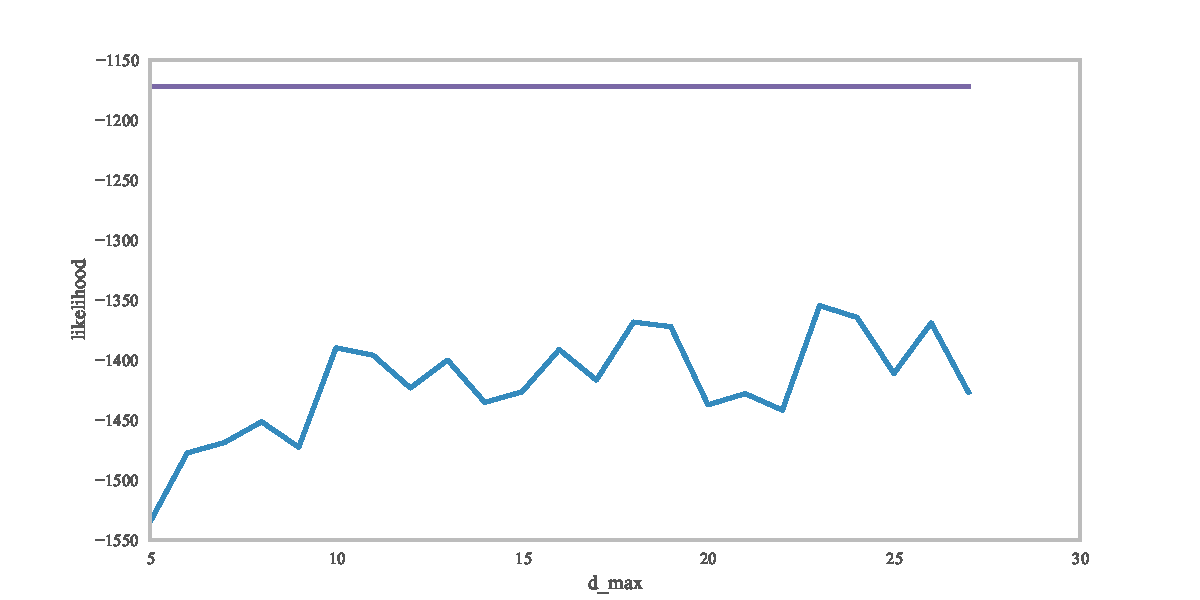
\includegraphics[width=0.8\textwidth]{../pic/likelihood_over_dmax.pdf}
	\caption{Mean likelihood over samples after burn-in as the range of possible durations increases (blue line). Shown for comparison is the mean likelihood of the beam sampler (purple line)}
\end{figure}


\section*{Reviwewr 2}

We thank the reviwer for their commenets, we have adressed the typos. 

\section*{Reviewer 3}

Reviwer 3 has highlighted two omissions in the paper. The first was that we did not make clear the fact that the Explicit Duration HMM is a type of Hidden Semi Markov Model, which is now made clear in the second paragraph of the introduction, along with an additional citation to an HSMM review detailing the relationship. The second was that we did not report on the results of the transition rate parameter estimates. While we do not report any detailed results for these parameters, as they are not the focus of the paper, we have made sure to report that this estimation is done. The reader is able to reproduce our experiments using the code online for more detailed investigation if necessary. 

We were unable to include all of the references mentioned due to the space limitations of the paper, however we have made sure to include one speech-synthesis paper, also suggested by revier 1, by Zen et al to make sure this application area is represented in the text. 

\section*{Reviwer 4}

We thank the reviewer for their comments, and have fixed the typos. 
\end{document}